    \section{Politics - Book I}

        \subsection{Introduction: The Polis and the Oikos}

            One of Aristotle’s key distinctions in Politics Book I is between the \textit{polis} (the city or political community) and the \textit{oikos} (the household or family). For the ancient Greeks, these two spheres represented fundamentally different realms of human activity:
    
                \begin{definition}[oikos]
                    The \textit{oikos} is the sphere of necessity—it deals with survival, daily needs, and household management.
                \end{definition}
    
                \begin{definition}[polis]
                    The \textit{polis} is the sphere of freedom—it aims at enabling people to live the good life, one marked by virtuous activity and flourishing.
                \end{definition}

            \subsubsection{A Central Question}

                \begin{quote}
                    Should the state be managed as an enterprise or not? Should an entrepreneur manage the state as if it were his enterprise?
                \end{quote}

                This question highlights a tension still relevant today: can (or should) the principles of economic management (focused on profit, efficiency, resource allocation) govern the political realm (focused on justice, common good, and the flourishing of citizens)?
                
                Aristotle’s answer—developed throughout his Politics—is that the methods of running a household economy (oikos) and the methods of running a political community (polis) are necessarily different. Politics, for Aristotle, is not merely a larger-scale version of household management.
\newpage
            \subsection{Digression: Hannah Arendt}

                Hannah Arendt (1906–1975) was a 20th-century political theorist whose works often draw on ancient Greek thought. Two of her major works are:
\vspace{-0.05cm}
                    \begin{itemize}
                        \item \textit{The Origins of Totalitarianism} (1951) – An analysis of totalitarian regimes (Nazi Germany, Stalinist Russia), focusing on how they subverted the public realm and destroyed the capacity for genuine political action.
                        \item \textit{The Human Condition} (1958) – An exploration of what it means to be human in the modern age, distinguishing different kinds of human activities (labor, work, and action) and reflecting on the modern eclipse of authentic political life.
                    \end{itemize}

                \subsubsection{Arendt on “Political Economy”}

                    Arendt famously claimed that the term “\textbf{political economy}” is an \textit{oxymoron}. \textbf{Why?} In antiquity, politics and economics were understood to be distinct spheres:
                            \begin{itemize}
                                \item \textbf{Economics} (oikonomia) is the management of the household (oikos), governed by necessity and the administration of resources.
                                \item \textbf{Politics} (the life of the polis) is the realm of public freedom, speech, and action, dedicated to matters of justice and the common good.
                            \end{itemize}

                    For Arendt, and following Aristotle, conflating these two realms—treating the political community as though it should be run by the same principles as a household or enterprise—distorts the essence of politics, which involves deliberation about the just and the unjust, the good and the bad, and the shared life of citizens.
\vspace{-0.25cm}
                \subsubsection{Arendt’s Three Human Activities}

                    In \textit{The Human Condition}, Arendt distinguishes three fundamental human activities:
\vspace{-0.05cm}
                        \begin{enumerate}
                            \item \textbf{Animal laborans} (the laboring animal)
                                \begin{itemize}
                                    \item Concerned with biological life (eating, sleeping, reproducing).
                                    \item Its tasks are repetitive and cyclical, tied to necessity.
                                \end{itemize}
                            \item \textbf{Homo faber} (the maker or builder)
                                \begin{itemize}
                                    \item Concerned with production or fabrication—crafting things that endure beyond their maker’s lifespan (e.g., art, tools, buildings).
                                    \item Gives the world a degree of permanence and durability.
                                \end{itemize}
                            \item \textbf{Zoon politikon} (the political animal)
                                \begin{itemize}
                                    \item Concerned with action (praxis) and speech, particularly in the public realm.
                                    \item Seeks the good life through debate, deliberation, and collective decision-making, embodying the classic Greek notion of full human flourishing.
                                \end{itemize}
                        \end{enumerate}

                    \begin{remark}
                        In ancient Greece, these spheres were more distinctly separated. Today, modern societies often conflate or subordinate the political (the realm of freedom and debate) to the economic (the realm of necessity and consumption)
                    \end{remark}

                \subsection{Succession and Priority}

                    \begin{remark}[Succession]
                        \textit{oikos} \(\rightarrow\) \textit{kòme} \(\rightarrow\) \textit{polis}
                    \end{remark}
            
                    Aristotle observes a developmental sequence in human communities: from the family (\textit{oikos}), to the village (\textit{kòme}), and finally to the city-state (\textit{polis}). However, he also asserts that the polis is by nature prior to the household and the individual (a statement he elaborates on in Politics 1253a).

                    While it might seem that the household comes “first,” Aristotle’s point is that the fully realized form of human association—the polis—logically and ontologically precedes the household in importance: only within a polis can human beings achieve the higher ends of justice and virtue.
            

        \section{Zoon Politikon}

            In Book I of the Politics, Aristotle famously argues that human beings are political animals (zoon politikon) more so than any other gregarious or social creatures. Unlike bees or ants, which also cooperate, humans have a unique capacity for logos—reasoned speech. This capacity allows us to discuss justice, goodness, advantageous vs. harmful, and other moral distinctions in ways that mere instinctual signalling cannot.

            \begin{quote}
                It is thus clear that man is a political animal (zoon politikon), in a higher degree than bees or other gregarious animals. Nature, according to our theory, makes nothing in vain; and man alone of the animals is furnished with the faculty of language. 
                
                The mere making of sounds serves to indicate pleasure and pain, and is thus a faculty that belongs to animals in general: their nature enables them to attain the point at which they have perceptions of pleasure and pain, and can signify those perceptions to one another.

                But language serves to declare what is advantageous and what is the reverse, and it is the peculiarity of man, in comparison with other animals, that he alone possesses a perception of good and evil, of the just and the unjust, and other similar qualities; and it is association in these things which makes a family (oikos) and a city (polis).

                (Aristotle, Politics 1253a7-18)
            \end{quote}

                \subsubsection{The Role of Language (Logos)}
    
                    \begin{itemize}
                        \item Mere sounds are shared by many animals, indicating pleasure and pain (e.g., growls, screeches).
                        \item Speech (logos) in the human sense involves the articulation of concepts such as justice and injustice, good and evil—a moral dimension unique to human beings.
                    \end{itemize}
    
                    Hence, the capacity for public discourse (deliberation, persuasion, debate) is the foundation of political life. This is why the community that arises from such discourse—the polis—is crucial for human flourishing: we need a public space in which to exercise our capacity to debate justice and the good.

            \subsection{Polis and Oikos}

                \begin{quote}
                    We may now proceed to add that the city (polis) is prior in the order of nature to the family (oikos) and the individual. The reason for this is that the whole is necessarily prior to the part. If the whole body is destroyed, there will not be a foot or a hand, except in that ambiguous sense in which one uses the same word to indicate a different thing, as when one speaks of a ‘hand’ made of stone…

                    (Aristotle, Politics 1253a18-25)
                \end{quote}

                    Aristotle here uses a biological analogy: just as a hand cannot fully exist as a hand if severed from the body, so the household and individual cannot truly exist (in their proper form) apart from the city. This does not deny the importance of families or individuals; rather, it emphasizes that the complete flourishing of each part depends on the whole of which it is a part.

                    \subsubsection{Reversal of Our Usual Intuition}

                        Modern political thought often treats the individual or household as the most fundamental social unit from which the city or state is built up. Aristotle reverses this, claiming the city is natural and logically prior: its presence is what allows families and individuals to function as they are meant to.

                    \subsubsection{On Justice Within the Oikos}

                        Aristotle does acknowledge that forms of justice exist even within the family and the household (for example, fair division of tasks, authority relations, etc.), but he insists that complete or perfect justice—the truly ethical-political sense of justice—can only be realized in a community that is organized for the common good and fosters moral virtue.

                \begin{remark}
                    Now the roles are inverted: the \textit{oikos} is not an \textit{oikos} if it is not part of a \textit{polis}
                \end{remark}

            \subsection{A Beast or a God}

                \begin{quote}
                    We thus see that the city exists by nature (physis) and that it is prior to the individual. For if the individual is not self-sufficient when he is isolated he will stand in the same relation to the whole as other parts do to their wholes. The man who is isolated, who is unable to share in the benefits of political association, or has no need to share because he is already self-sufficient, is no part of the city, and must therefore be either a beast or a god. 

                    (Aristotle, Politics 1253a25-b1)
                \end{quote}

                    This famous passage underscores the notion that a person who lives entirely outside the political community is either:

                    \begin{itemize}
                        \item \textbf{Less than fully human} (a “beast”), if he lacks the rational and moral capacity to engage with others in a city,
                        \item \textbf{More than human} (a “god”), if by some miracle he is self-sufficient and needs no political association whatsoever.
                    \end{itemize}

                \begin{quote}
                    Man, when perfected, is the best of animals; but if he be isolated from law and justice he is the worst of all. Injustice is all the graver when it is armed injustice; and man is furnished from birth with weapons which are intended to serve the purposes of wisdom and goodness, but which may be used in preference for opposite ends.

                    (Aristotle, Politics 1253a25-b1)
                \end{quote}

                In other words, human beings possess language, reason, and moral agency, and these can be used to promote virtue—or to commit grave injustices. The city, with its laws and communal deliberations, is what orients humans toward the good life, restraining our base impulses and fostering ethical development.

            \subsection{The Virtue of Justice}

                \begin{quote}
                    That is why, if he be without goodness [of mind and character], he is a most unholy and savage being, and worse than all others in the indulgence of lust and gluttony. The virtue of justice belongs to the city; for justice is an ordering of the political association, and the virtue of justice consists in the determination of what is just.

                    (Aristotle, Politics 1253a25-b1)
                \end{quote}

                \subsubsection{Justice as a Practice}

                    For Aristotle, virtue (including justice) is not simply a set of rules or abstract propositions; it is a habit or disposition cultivated through practice and participation in communal life. Justice in particular:

                    \begin{itemize}
                        \item \textbf{Cannot be decreed by fiat alone}; it emerges through deliberation and habituation.
                        \item \textbf{Requires an active engagement of citizens} in lawmaking and judging what is just or unjust.
                    \end{itemize}

                    Hence, Aristotle links ethics and politics very closely. We cannot fully understand or exercise justice outside of a political community dedicated to promoting the common good. Because justice aims at proportional equality (treating equals equally and unequals unequally according to their merits), it involves a kind of mathematical proportion—yet it is not purely numerical. It also requires practical wisdom (\textit{phronesis}) to discern what is fair in particular circumstances.

        \section*{L1.1 - Additional Context and Conclusions}
                    
            \begin{remark}[Aristotle’s Context]
                Written in the 4th century BCE, in the era of the Greek polis, Politics reflects a time when the city-state was the primary political unit. Participation in civic life (legislative assemblies, courts, festivals) was central to Greek identity.
            \end{remark}

            \begin{remark}[Modern Implications]
                In contemporary political theory, the question of whether we can or should run the state like a business or a household remains crucial. Many debates around neoliberalism, public policy, welfare, and governance hinge on whether the logic of the market (efficiency, profit) should override or be subordinated to political considerations (justice, rights, common good).
                
                The idea that “man is a political animal” remains deeply relevant to democratic theory—human beings thrive in communities where they can debate and define what is just, rather than purely living by private or economic dictates.
            \end{remark}

            \begin{remark}[Hannah Arendt’s Contribution]
                Arendt’s emphasis on the public realm of action and speech, distinct from the private realm of labour and necessity, revives some of Aristotle’s concerns for the modern age. In her view, \textbf{totalitarianism emerges partly from the collapse} or destruction \textbf{of the public-political realm}, where genuine debate and individual conscience should operate.
            \end{remark}

            \begin{remark}[Justice and Education]
                Aristotle sees education in virtue as inseparable from the structure of the polis itself. The laws and customs of a well-ordered polis teach citizens to be just through practice.
                
                \textbf{Justice is thus not only a theoretical virtue} but one requiring political institutions that habituate citizens to act ethically.
            \end{remark}

        \section[Nicomachean Ethics -- Book V]{Nicomachean Ethics -- \href{https://drive.google.com/file/d/1uxgtqKid4c8Lfgl5nKP3dV5EZDR9dZ-L/view?usp=share_link}{Book V}}

            \subsection{Preamble -- Two Kinds of Justice}

                Aristotle famously distinguishes between two primary kinds of justice:
                \begin{enumerate}
                  \item \textbf{Distributive justice}
                  \item \textbf{Rectificatory (or corrective) justice}
                \end{enumerate}

                These two types address different contexts: one pertains to the fair distribution of common goods or honors among members of a community; the other pertains to righting wrongs or correcting imbalances in individual transactions or harms.

                \subsubsection{Unjust or Unequal}

                    Aristotle observes that the unjust person is unfair---he acts in ways that create or maintain inequality. Conversely, what is just is a kind of equality or fairness. Since a virtue aims at a mean and unfairness is an excess or deficiency, justice, too, must be a mean. More concretely:
                    \begin{itemize}
                      \item If the unjust is \textbf{unequal}, then the just must be \textbf{equal}.
                      \item Equality is a kind of \textbf{mean} between the extremes of ``too much'' and ``too little.''
                    \end{itemize}

                    In Book II, Aristotle uses the example of \textit{cowardice, courage, and temerity} to illustrate how virtue is a mean between extremes. Analogously, in Book V, \textit{justice} is the mean between the extremes of taking too much (excess) and taking too little (deficiency).

                \subsubsection{The Mean}

                    \begin{center}
                        \textbf{Cowardice -- Courage -- Temerity}
                    \end{center}
                    
                    This triad from Book II serves as a helpful analogy. For justice specifically, imagine an overreach (excess, taking or giving too much) and a shortfall (deficiency, taking or giving too little). Justice, then, stands in the middle as the balanced, fair position.

            \subsection{Four Terms}

                Because equality involves balancing at least two parties and their two shares (or goods, resources, etc.), Aristotle says that doing justice will require dealing with four terms:
                \begin{enumerate}
                  \item Two persons (the parties involved)
                  \item Two shares (the goods or resources to be allocated or rectified)
                \end{enumerate}

                Insofar as it is a mean, justice lies between excess and deficiency; insofar as it is \textit{equal}, it involves at least two people and two shares; insofar as it is \textit{just} for those people, it is relative to them.

                \begin{remark}[Unequal persons, unequal shares]
                    If persons differ in status, merit, or contribution, their shares should also reflect that inequality (and vice versa). Quarrels arise when equal persons receive unequal shares, or when unequal persons receive equal shares.
                \end{remark}

                \subsubsection{Merit}

                    Aristotle underscores that justice must also track \textbf{merit} or \textbf{desert} (in Greek, \emph{axia}). The core principle of distributive justice is that people should receive shares in proportion to their merit or contribution. What exactly ``merit'' means can vary (it could be virtue, wealth, contribution to the common good, etc.), but the central idea is that justice must be proportional.

            \subsection{Distributive Justice}

                \begin{proposition}
                    Distributive justice deals with how common goods (like wealth, honors, or resources) are distributed among members of a community.
                \end{proposition}
                 
                Aristotle describes this as a \textbf{geometrical proportion}:
                \[
                A : B \;=\; C : D 
                \quad \text{and} \quad
                A : C \;=\; B : D.
                \]
                
                \begin{itemize}
                  \item $A$ and $B$ are the people (or their respective degrees of merit).
                  \item $C$ and $D$ are the shares they receive.
                \end{itemize}
                
                \begin{example}
                    A classic example might be awarding prizes in a poetry contest:
                    \begin{enumerate}
                      \item $A$ = the best poet, $B$ = the second-best poet
                      \item $C$ = a gold crown, $D$ = a silver crown
                    \end{enumerate}
                \end{example}

                Hence, the best poet is to the gold crown as the second-best poet is to the silver crown. The distribution is ``just'' or proportional when each person's share corresponds to their relative standing or merit.

                \subsubsection{Geometrical Proportion}

                    \begin{quote}
                    \textit{``What is just in distribution\ldots mathematicians call this kind of proportion \textbf{geometrical}.''}
                    \end{quote}

                    \begin{itemize}
                      \item In \textit{geometrical} proportion, we look at ratios, so that if person A is twice as deserving as person B, A should receive twice the share.
                      \item The ``mean'' in distributive justice is found by balancing these proportional relationships, not by splitting resources \textit{equally} across the board, but by splitting them \textit{proportionally} to each person's status or merit.
                    \end{itemize}

            \subsection{Rectificatory Justice}

                \begin{proposition}
                    Rectificatory (or corrective) justice addresses imbalances or harms arising from both \textbf{voluntary} and \textbf{involuntary} transactions.
                \end{proposition}
                
                Unlike distributive justice, which is guided by a geometrical proportion, rectificatory justice deals with \textbf{arithmetical} proportion.

                \begin{itemize}
                  \item \textbf{Voluntary transactions}: buying, selling, lending, hiring, etc.
                  \item \textbf{Involuntary transactions}: theft, assault, fraud, murder, and other harms inflicted without mutual consent.
                \end{itemize}

                \subsubsection{Arithmetical Proportion}

                    In these situations, the law aims at restoring a balance that has been \textit{disrupted} by one party's wrongful gain and the other's corresponding loss. Whether the parties are ``good'' or ``bad'' in character does not matter to the law; it looks only to the fact that an injury or injustice occurred, and it wants to ``right'' that wrong:

                    \begin{quote}
                    \textit{``For it makes no difference whether it is a good person who has defrauded a bad or a bad person a good\ldots The law looks only to the difference made by the injury.''}
                    \end{quote}

                    Hence, rectification tries to \textbf{equalize} by subtracting the unfair gain and compensating the victim's loss---restoring both parties to a fair baseline.

                \subsubsection{The Role of the Judge}

                    Because rectificatory justice is about \textit{restoring} an equilibrium, the judge's role is crucial. The judge:
                    \begin{enumerate}
                      \item Assesses the \textit{damage} (the difference between what happened and what should have been).
                      \item Imposes a \textit{penalty} or requires compensation to remove the excess gain from the wrongdoer and remedy the victim's loss.
                    \end{enumerate}

                    Aristotle likens this to a line with unequal segments: you subtract from the longer segment and add to the shorter segment until you reach the midpoint.

                \subsubsection{Loss and Gain}

                    Aristotle uses the language of ``loss'' and ``gain'' metaphorically:
                    \begin{itemize}
                      \item When one party takes more than what is legitimately theirs, they have a \textbf{gain}.
                      \item The other party suffers a \textbf{loss}, having less than they started with or less than is right.
                    \end{itemize}
                    
                    Rectification restores them to an \textbf{equal} position---arithmetically, each party ends up with what they would have had if no injustice had occurred.

            \subsection{The Mean}

                What is \textit{equal} (the just outcome) is the mean between the greater and the less, according to \textbf{arithmetical} proportion. This applies especially to rectificatory justice, where you add or subtract precisely the difference that caused the imbalance.

                Aristotle provides geometric illustrations, showing how we find the middle by subtracting from one side and adding to the other until an equilibrium is established.

                \begin{example}

                    Let the lines AA', BB' and CC' be equal to one another.
    
                        \begin{center}
                            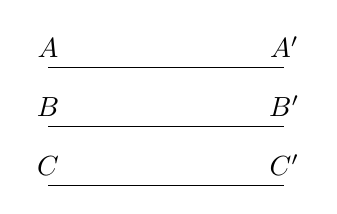
\begin{tikzpicture}[scale=0.75]
                              % Line for A--A'
                              \draw (0,0) -- (4,0);
                              \node[above]  at (0,0)   {$A$};
                              \node[above] at (4,0)   {$A'$};
                            
                              % Line for B--B'
                              \draw (0,-1) -- (4,-1);
                              \node[above]  at (0,-1)  {$B$};
                              \node[above] at (4,-1)  {$B'$};
                            
                              % Line for C--C'
                              \draw (0,-2) -- (4,-2);
                              \node[above]  at (0,-2)  {$C$};
                              \node[above] at (4,-2)  {$C'$};
                            \end{tikzpicture}
                        \end{center}
                        
                        \vspace{1em}
    
                        From the line AA', let the segment AE be subtracted:
    
                        \begin{center}
                            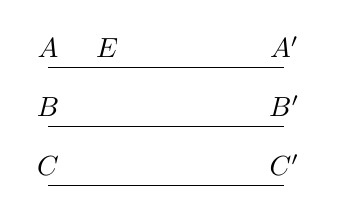
\begin{tikzpicture}[scale=0.75]
                              % A--E--A'
                              \draw (0,0) -- (4,0);
                              \node[above]  at (0,0)   {$A$};
                              \node[above] at (1,0)   {$E$};  % Place E somewhere between A and A'
                              \node[above] at (4,0)   {$A'$};
                            
                              % B--B'
                              \draw (0,-1) -- (4,-1);
                              \node[above]  at (0,-1)  {$B$};
                              \node[above] at (4,-1)  {$B'$};
                            
                              % C--C'
                              \draw (0,-2) -- (4,-2);
                              \node[above]  at (0,-2)  {$C$};
                              \node[above] at (4,-2)  {$C'$};
                            \end{tikzpicture}
                        \end{center}
                        
                        \vspace{1em}
    
                        and the segment CD added to the line CC', so that the whole line DCC' exceeds the line EA' by the segment CD and the segment CF; thus it exceeds the line BB' by the segment CD.
    
                        \begin{center}
                            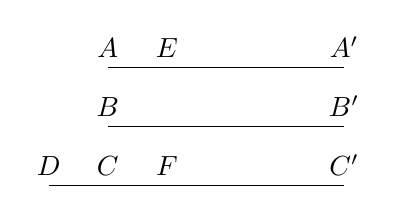
\begin{tikzpicture}[scale=0.75]
                              % A--E--A'
                              \draw (0,0) -- (4,0);
                              \node[above]  at (0,0)   {$A$};
                              \node[above] at (1,0)   {$E$};
                              \node[above] at (4,0)   {$A'$};
                            
                              % B--B'
                              \draw (0,-1) -- (4,-1);
                              \node[above]  at (0,-1)  {$B$};
                              \node[above] at (4,-1)  {$B'$};
                            
                              % D--C--F--C'
                              \draw (-1,-2) -- (4,-2);
                              \node[above]  at (-1,-2)  {$D$};
                              % Choose positions for C and F
                              \node[above] at (0,-2)  {$C$}; 
                              \node[above] at (1,-2)  {$F$};
                              \node[above] at (4,-2)  {$C'$};
                            \end{tikzpicture}
                        \end{center}
                        
                    \end{example}

\newpage

            \subsection{Two Kinds of Justice}

                \begin{definition}
                    \textbf{Distributive Justice} (Geometrical Proportion)
                    \begin{itemize}
                      \item Involves \textit{unequal} people (e.g., differing in merit) who should receive \textit{unequal} shares in proportion to their respective deserts.
                      \item Formula: $A : B = C : D$.
                    \end{itemize}
                \end{definition}

                \begin{definition}
                    \textbf{Rectificatory Justice} (Arithmetical Proportion)
                    \begin{itemize}
                      \item Involves \textit{equal persons} under the law who must be restored to a fair baseline when an injustice has occurred.
                      \item The judge ``corrects'' or ``rectifies'' by \textbf{subtracting} from the wrongdoer's gain and \textbf{adding} to the victim's loss.
                    \end{itemize}
                \end{definition}

                \subsubsection{Loss and Gain (revisited)}

                    \begin{itemize}
                      \item \textbf{Derivation}: The ideas of ``loss'' and ``gain'' come from \textit{voluntary exchange}, where one typically does not want to end up with less value (loss) or more than one's due (gain).
                      \item \textbf{Balance}: In just exchanges, each party ends with the value equivalent to what they began with, or at least with an agreed-upon equivalence of goods, services, or money.
                    \end{itemize}

            \subsection{Transactions}

                Aristotle divides transactions into:
                \begin{enumerate}
                  \item \textbf{Involuntary transactions}
                    \begin{itemize}
                      \item Examples: theft, assault, homicide, fraud, etc.
                      \item These necessitate the intervention of a judge or legal remedy to \textit{correct} (rectify) the imbalance.
                    \end{itemize}
                  \item \textbf{Voluntary transactions}
                    \begin{itemize}
                      \item Examples: commercial exchanges, renting, hiring, etc., where both parties consent.
                      \item These transactions \textit{can} still lead to disputes about ``gain'' and ``loss'' if the agreement is not honored or if one party defrauds the other.
                    \end{itemize}
                \end{enumerate}

                \subsubsection{Reciprocity}

                    Some philosophers (like the Pythagoreans) held that \textbf{reciprocity} (\emph{an eye for an eye}) is justice in an unqualified sense. However, Aristotle notes that strict reciprocity (literal tit-for-tat) does not accurately capture \textit{distributive} or \textit{rectificatory} justice, especially in cases where the parties' status is not the same (e.g., a citizen striking a magistrate might be punished more severely than if the roles were reversed).

                \subsubsection{Proportionate Reciprocation}\label{L1.2:Proportionate_Reciprocation}
                
                    Aristotle explains that in \textit{voluntary exchanges}, there is a form of justice he calls \textbf{``reciprocity in accordance with proportion.''} It is not mere equality of retaliation or transaction, but a reciprocal balance that accounts for the relative value of goods or services:
                    
                    \begin{quote}
                    If \textbf{A} is a builder and \textbf{B} is a shoemaker, and we want to exchange a house for shoes, the two must be \textit{commensurable} in a certain proportion so that the exchange is fair.
                    \end{quote}

        \section{A Third Kind of Justice}

            In addition to \textbf{distributive} and \textbf{rectificatory} justice, Aristotle explores a \textbf{third} concept often referred to as:
            \begin{quote}
            \[
            \text{\textit{antipeponthos kat' analogían}}
            \]
            \[
            \text{reciprocity in accordance with proportion.}
            \]
            \end{quote}

            This describes a kind of \textbf{proportional reciprocity} that arises especially in \textit{economic exchanges}, serving as the glue that holds a society together by rewarding good with good and returning bad with bad---yet doing so in proportion to the relative values or severity involved.

                \subsubsection{Proportionate Reciprocation}

                    When people engage in market exchanges, they must equate different goods in order to trade. Aristotle highlights:
                    \begin{itemize}
                      \item \textbf{A} (the builder)
                      \item \textbf{C} (a house)
                      \item \textbf{B} (the shoemaker)
                      \item \textbf{D} (shoes)
                    \end{itemize}

                    A fair exchange occurs when \textbf{A} receives from \textbf{B} a quantity of goods (shoes) that is proportionate in value to what \textbf{A} gives (a house). If one person's goods are inherently more valuable, the exchange ratio must reflect that.

            \subsection{Measure (The Role of Money)}

                Because houses, shoes, and other goods are not easily compared, society uses \textbf{money} as a conventional measure:
                \begin{enumerate}
                  \item Money acts as a \textbf{mean}, making goods and services \textbf{commensurable}.
                  \item It provides a universal measure of value so that we can compare ``how many shoes equal one house.''
                \end{enumerate}
                
                Aristotle derives the Greek word for money, \emph{nomisma}, from \textit{nomos} (law or convention), to emphasize that money's value is established by collective agreement. Without money, trade would rely on barter, which complicates finding fair ratios (how many shoes per house?).

                \subsubsection{Proportional Reciprocity in Practice}

                    It is not that two doctors exchange services, but rather a farmer and a doctor, or a builder and a shoemaker. Because these parties produce different and \textit{unequal} things, there must be a standardized method (money) to equate and balance their transactions. This fosters \textbf{social cohesion}: people exchange goods or services in proportion to their value, keeping relationships functional and the city unified.

        \section*{L1.2 -- Conclusions}

            Aristotle's discussion in Book V of the \textit{Nicomachean Ethics} reveals how \textbf{justice} can be understood in several overlapping senses:
            \begin{enumerate}
              \item \textbf{Distributive justice} deals with proportional allocations to \textbf{unequal} persons, according to their merit (geometrical proportion).
              \item \textbf{Rectificatory justice} addresses the correction of wrongs through \textbf{arithmetical} proportion, treating the parties as equals before the law, subtracting from the wrongdoer's excess and compensating the victim's loss.
              \item \textbf{Proportionate reciprocity} (sometimes taken as a \textbf{third} kind of justice) emphasizes fair exchange in economic or social transactions, achieved through a \textbf{proportional} equality rather than mere equality. Money becomes a key instrument for measuring and making commensurable the goods or services exchanged.
            \end{enumerate}
            
            \begin{remark}
                In \textbf{distributive} justice, differences in people's status or merit lead to \textbf{unequal} allocations that are still fair because they are \textit{proportionate}. In \textbf{rectificatory} justice, the parties are treated as \textbf{equals} in the sense that the law imposes a correction for the wrongdoing. In \textbf{exchange}, people's different products or services must be brought into a \textbf{proportionate} equality so that trade can occur fairly.
            \end{remark}

            \begin{remark}[Why we use mathematics in \ref{L1.2:Proportionate_Reciprocation}]
                From the greek ``\textit{mathēmatikē}'', from the base of ``\textit{manthanein}'', to learn. It is simply more logical to argue via the use of math, as it allows us to uncover and argue for something that is already known.
            \end{remark}
            
            Aristotle's overarching conclusion is that although all three share something in common---namely, the idea of \textbf{balance} or \textbf{mean}---they apply in different realms (distribution of public goods, correction of private harms, and exchange of goods/services). Where \textbf{distributive justice} and \textbf{rectificatory justice} ``rectify'' imbalances by either awarding shares in proportion to merit or compensating losses, \textbf{proportionate reciprocity} emphasizes mutual benefit and the cohesive power of fair trade in the city.
            
            Thus, differences are recognized---merit, wrongdoing, product value---but justice seeks to bring them into a \textbf{measured} or \textbf{proportional} equilibrium, preserving harmony and fairness in social life.
